\chapter{Suhu dan Termometer}\label{ch:g3:temperature-thermometers}

Dua musim dingin yang lalu, tiga mangkuk air menipu kedua tanganmu:
air yang sama terasa hangat bagi tangan yang satu dan sejuk bagi yang
lain. Waktu itu kita berjanji bahwa suatu hari sebuah alat akan
menyelesaikan pertengkaran semacam itu. Inilah dia --- \omterm{def:g3:temperature-thermometers:temperature}{termometer},
hakim kaca kecil yang mengubah panas dan dingin menjadi sebuah
bilangan.

\section{Mengapa perabaan tidak cukup}

\begin{example}[Para hakim yang tidak adil]\label{ex:g3:temperature-thermometers:unfair}
Perabaan menghakimi dengan tidak adil pada setiap musim: perosotan
logam terasa lebih dingin daripada bangku kayu yang berdiri di tempat
teduh yang sama; air suam-suam kuku terasa hangat bagi tangan yang
dingin dan sejuk bagi tangan yang hangat; dan sesudah bermain kereta
salju, lorong yang sejuk pun terasa hangat sekali. Untuk membandingkan
panas dan dingin dengan jujur --- antarruangan, antarhari, antarorang
--- kita memerlukan hakim yang tidak pernah berubah pikiran: sebuah
alat.
\end{example}

\section{Termometer dan derajatnya}

\begin{definition}[Suhu]\label{def:g3:temperature-thermometers:temperature}
Bilangan yang menyatakan tepat seberapa panas atau dingin sebuah benda
disebut \emph{suhu}\index{suhu} benda itu. Makin tinggi bilangannya,
makin panas bendanya; makin rendah bilangannya, makin dingin. Suhu
diukur dalam \emph{derajat Celsius}\index{derajat Celsius}, ditulis
\unit{\celsius}, dengan sebuah \emph{termometer}\index{termometer}.
\end{definition}

\begin{proposition}[Dua tonggak air]\label{prop:g3:temperature-thermometers:milestones}
Skala Celsius dipatok pada dua perubahan wujud air yang besar:
\begin{enumerate}
  \item pada \qty{0}{\celsius}, air \omterm{def:g2:ice-water-steam:meltfreeze}{membeku} menjadi es (dan es
        \omterm{def:g2:ice-water-steam:meltfreeze}{mencair});
  \item pada \qty{100}{\celsius}, air mendidih menjadi uap.
\end{enumerate}
Di antara kedua tonggak itu, skalanya dipotong menjadi $100$ derajat
yang sama besar --- sebuah tangga berundak kecil dari es sampai uap.
\end{proposition}

\begin{omfigure}
\begin{tikzpicture}[scale=0.85]
  \draw[thick] (0.5,0) rectangle (1.1,6.0);
  \draw[thick] (0.8,0) circle (0.42);
  \fill[omThm, opacity=0.7] (0.8,0) circle (0.34);
  % scale: 0 C at y=0.6, one unit of height per 20 C -> 25 C at y=1.85
  \fill[omThm, opacity=0.7] (0.62,0.05) rectangle (0.98,1.85);
  \foreach \y/\t in {0.6/0, 1.6/20, 2.6/40, 3.6/60, 4.6/80, 5.6/100} {
    \draw (1.1,\y) -- (1.35,\y);
    \node[right, font=\footnotesize] at (1.4,\y) {$\t$};
  }
  \foreach \y in {1.1, 2.1, 3.1, 4.1, 5.1} {
    \draw (1.1,\y) -- (1.25,\y);
  }
  \node[right, font=\small, omDef] at (2.6,0.6)
    {\qty{0}{\celsius}: air membeku};
  \node[right, font=\small] at (2.6,1.85)
    {\qty{25}{\celsius}: bacaan ini};
  \node[right, font=\small, omThm] at (2.6,5.6)
    {\qty{100}{\celsius}: air mendidih};
  \draw[-Stealth, omExo] (2.5,1.85) -- (1.05,1.85);
\end{tikzpicture}

{\small Sebuah \omterm{def:g3:temperature-thermometers:temperature}{termometer}: \omterm{def:g3:solids-liquids-gases:liquid}{zat cair} merahnya memanjat ketika
dihangatkan. Di sini ia berhenti pada tanda $25$ --- \omterm{def:g3:temperature-thermometers:temperature}{suhunya}
\qty{25}{\celsius}.}
\end{omfigure}

\begin{example}[Cara kerja sang hakim kaca]\label{ex:g3:temperature-thermometers:works}
Di dalam tabung tipis \omterm{def:g3:temperature-thermometers:temperature}{termometer} terperangkap \omterm{def:g3:solids-liquids-gases:liquid}{zat cair} berwarna.
Kehangatan membuat \omterm{def:g3:solids-liquids-gases:liquid}{zat cair} itu memuai sedikit saja --- dan di dalam
tabung yang begitu tipis, pemuaian yang sedikit sudah mendorong
kolomnya naik dengan jelas. Dingin menyusutkannya kembali. \omterm{def:g3:solids-liquids-gases:liquid}{Zat cair}
itu tidak dapat ditipu seperti tangan: ia memuai sama untuk kehangatan
yang sama, hari ini, besok, bagi siapa pun.
\end{example}

\begin{omfigure}
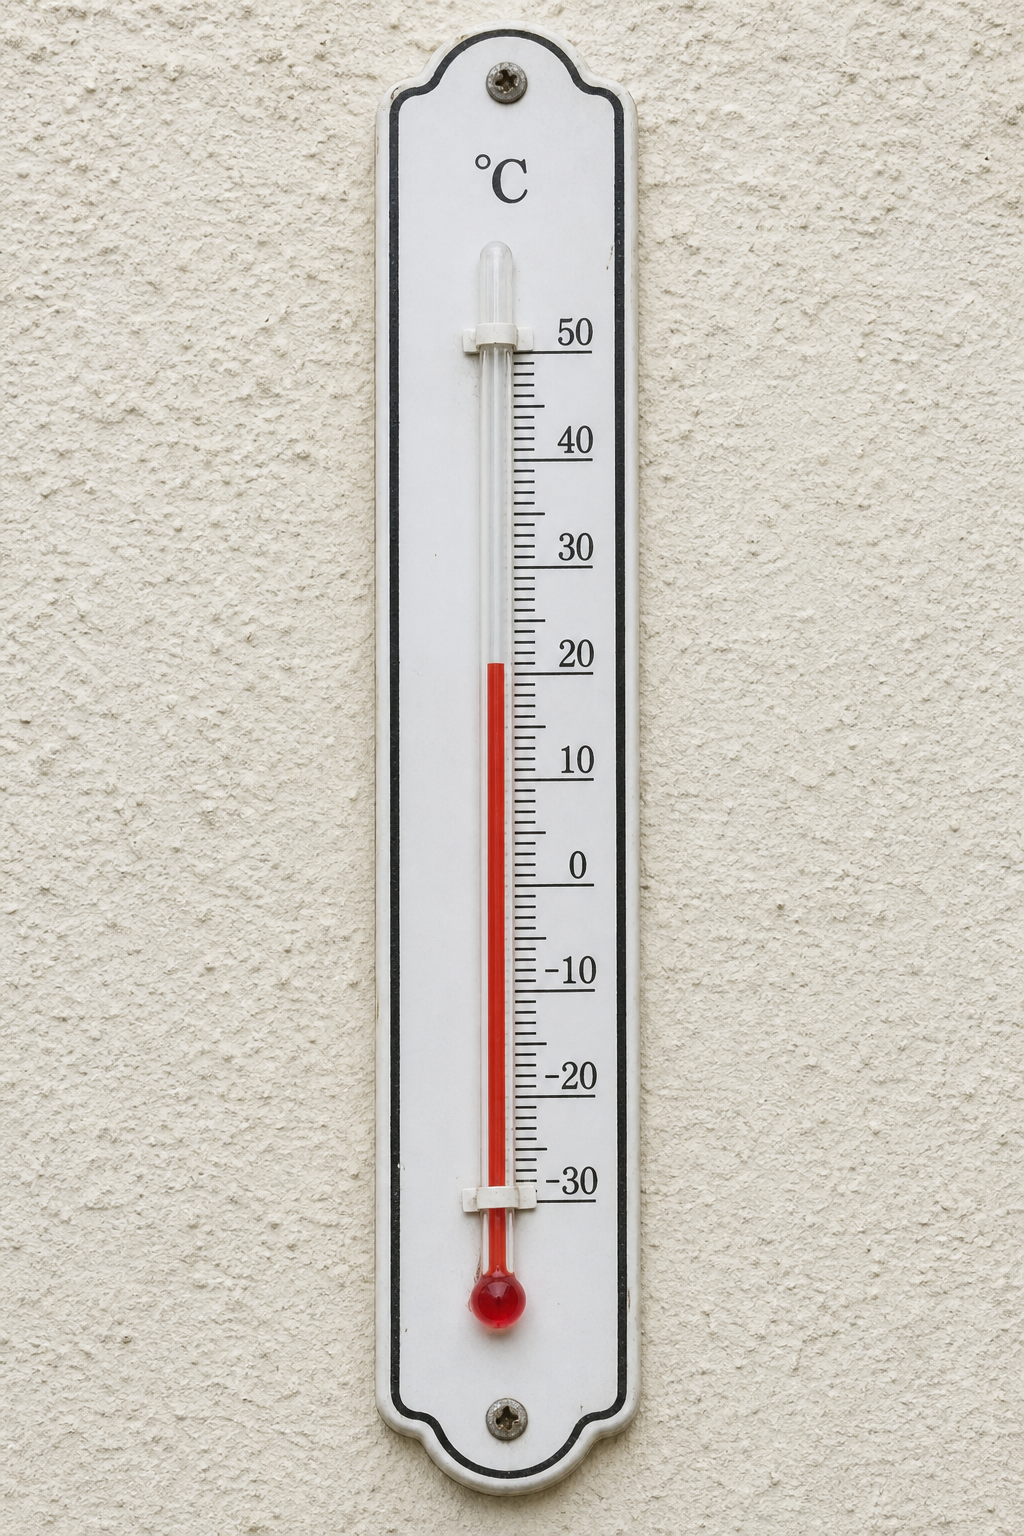
\includegraphics[width=0.3\linewidth]{images/book1/ai/g3-thermometer-outdoor.png}

{\small \omterm{def:g3:temperature-thermometers:temperature}{Termometer} sungguhan pada dindingnya: kolom merahnya memanjat skala, dan siapa pun yang membaca tandanya mendapat bilangan yang sama.}
\end{omfigure}

\section{Membaca termometer}

\begin{method}[Membaca termometer]\label{met:g3:temperature-thermometers:read}
\begin{enumerate}
  \item Letakkan \omterm{def:g3:temperature-thermometers:temperature}{termometer} di tempat yang \omterm{def:g3:temperature-thermometers:temperature}{suhunya} ingin kamu ketahui
        --- di dalam air, di tempat teduh di luar rumah, di bawah
        lidah;
  \item \emph{tunggulah} --- \omterm{def:g3:solids-liquids-gases:liquid}{zat cairnya} perlu waktu untuk selesai
        memanjat atau turun; amati sampai ia berhenti bergerak;
  \item sejajarkan matamu dengan puncak kolomnya;
  \item bacalah bilangan pada tanda yang dicapai kolom itu, lalu
        tulislah dengan \omterm{def:g2:measuring-length:measure}{satuannya}: \qty{18}{\celsius}.
\end{enumerate}
Membaca terlalu cepat, atau dari arah menyerong, memberi bilangan yang
salah --- hakimnya jujur, tetapi ia harus ditanya dengan cara yang
benar.
\end{method}

\begin{example}[Suhu yang perlu dihafal]\label{ex:g3:temperature-thermometers:livedby}
Beberapa bilangan yang layak dihafal: ruangan yang nyaman kira-kira
\qty{20}{\celsius}; tubuhmu menjaga dirinya di sekitar
\qty{37}{\celsius}, baik pada musim panas maupun musim dingin (jauh di
atas itu berarti demam --- \omterm{def:g3:temperature-thermometers:temperature}{termometer} dokter tahu); lemari es menahan
sekitar \qty{4}{\celsius}; hari musim panas yang terik mencapai
\qty{30}{\celsius}; air mandi terasa nyaman di dekat
\qty{35}{\celsius}.
\end{example}

\begin{omfigure}
\begin{tikzpicture}[scale=0.85]
  \foreach \x/\h/\t/\name in {0/1.1/4/lemari es,
      3.0/2.1/20/ruangan yang nyaman, 6.0/3.0/37/tubuhmu,
      9.0/2.6/30/hari musim panas} {
    \draw[thick] (\x,0) rectangle ++(0.42,3.6);
    \fill[omThm, opacity=0.7] (\x+0.08,0.05) rectangle ++(0.26,\h);
    \node[above, font=\footnotesize] at (\x+0.21,3.65)
      {$\t$\,\unit{\celsius}};
    \node[below, font=\small, align=center] at (\x+0.21,-0.2) {\name};
  }
\end{tikzpicture}

{\small Empat \omterm{def:g3:temperature-thermometers:temperature}{suhu} yang akrab: makin tinggi kolomnya, makin panas
bendanya.}
\end{omfigure}

\section{Di bawah nol}

\begin{example}[Bilangan musim dingin]\label{ex:g3:temperature-thermometers:belowzero}
Pada pagi yang membekukan, kolomnya turun \emph{di bawah} tanda $0$.
Tanda-tandanya terus berlanjut ke bawah di sana, dan kita membacanya
dengan kata ``minus'': satu tanda di bawah nol adalah \emph{minus
satu} derajat, lima tanda di bawahnya adalah \emph{minus lima},
ditulis \qty{-5}{\celsius}. Bilangan minus lebih dingin daripada nol,
dan makin rendah bilangannya, makin keras bekunya: pagi $-10$
menggigit lebih dingin daripada pagi $-2$. Laporan cuaca
menyebutkannya setiap petang musim dingin.
\end{example}

\begin{remark}[Nol bukan berarti ``tidak ada'']\label{rem:g3:temperature-thermometers:zero}
Pada skala ini, $0$ tidak berarti ``tanpa \omterm{def:g3:temperature-thermometers:temperature}{suhu}'' --- ia sekadar tanda
tempat air \omterm{def:g2:ice-water-steam:meltfreeze}{membeku}, sebuah tonggak seperti rambu jalan. Cuaca dapat
lebih hangat daripada tonggak itu atau lebih dingin daripadanya;
\omterm{def:g3:temperature-thermometers:temperature}{termometer} hanya memberitahumu di sisi mana, dan berapa tanda jauhnya.
(Bilangan di bawah nol punya aritmetikanya sendiri --- pelajaran
matematikamu akan membahasnya dengan tuntas pada tahun yang lebih
tinggi.)
\end{remark}

\section{Latihan}

\begin{exercise}[$\star$]\label{exo:g3:temperature-thermometers:1}
Mengapa \omterm{def:g3:temperature-thermometers:temperature}{termometer} menjadi hakim panas dan dingin yang lebih adil
daripada tanganmu? Sebutkan satu cara tangan tertipu pada bab
sebelumnya.
\end{exercise}

\begin{exercise}[$\star$]\label{exo:g3:temperature-thermometers:2}
Pada \omterm{def:g3:temperature-thermometers:temperature}{suhu} berapa air \omterm{def:g2:ice-water-steam:meltfreeze}{membeku}? Mendidih? Kedua bilangan itu dalam
\omterm{def:g2:measuring-length:measure}{satuan} apa?
\end{exercise}

\begin{exercise}[$\star$]\label{exo:g3:temperature-thermometers:3}
Apa yang terjadi pada \omterm{def:g3:solids-liquids-gases:liquid}{zat cair} di dalam tabung tipis ketika \omterm{def:g3:temperature-thermometers:temperature}{termometer}
dihangatkan? Ketika didinginkan? Mengapa perubahan sekecil itu
terlihat begitu jelas?
\end{exercise}

\begin{exercise}[$\star$]\label{exo:g3:temperature-thermometers:4}
Sebutkan dua kesalahan yang diperingatkan oleh
\cref{met:g3:temperature-thermometers:read} ketika membaca \omterm{def:g3:temperature-thermometers:temperature}{termometer}.
\end{exercise}

\begin{exercise}[$\star$]\label{exo:g3:temperature-thermometers:5}
Pasangkan tiap benda dengan \omterm{def:g3:temperature-thermometers:temperature}{suhunya} yang paling mungkin ---
\qty{4}{\celsius}, \qty{20}{\celsius}, \qty{37}{\celsius},
\qty{100}{\celsius}: air mendidih; \ ruang keluarga yang nyaman;
\ bagian dalam lemari es; \ tubuhmu sendiri.
\end{exercise}

\begin{exercise}[$\star$]\label{exo:g3:temperature-thermometers:6}
\omterm{def:g3:temperature-thermometers:temperature}{Termometer} bak mandi terbaca \qty{35}{\celsius}; panci di atas kompor
terbaca \qty{100}{\celsius}. Mana yang lebih panas, dan amankah panci
itu disentuh? Berapa derajat panci itu lebih panas daripada bak mandi?
\end{exercise}

\begin{exercise}[$\star$]\label{exo:g3:temperature-thermometers:7}
\omterm{def:g3:temperature-thermometers:temperature}{Termometer} musim dingin menunjukkan kolomnya $3$ tanda di bawah nol.
Bagaimana kita mengucapkan dan menuliskan \omterm{def:g3:temperature-thermometers:temperature}{suhu} itu? Lebih dingin atau
lebih hangat daripada \qty{-8}{\celsius}?
\end{exercise}

\begin{exercise}[$\star$]\label{exo:g3:temperature-thermometers:8}
Kemarin \omterm{def:g3:temperature-thermometers:temperature}{termometer} kebun terbaca \qty{6}{\celsius} pada waktu sarapan
dan \qty{14}{\celsius} pada waktu makan siang. Berapa derajat pagi itu
menghangat?
\end{exercise}

\begin{exercise}[$\star$]\label{exo:g3:temperature-thermometers:9}
Genangan di trotoar berubah menjadi es semalaman. Apa yang dapat kamu
katakan tentang \omterm{def:g3:temperature-thermometers:temperature}{suhu} malam itu, tanpa \omterm{def:g3:temperature-thermometers:temperature}{termometer} sama sekali? Tonggak
mana yang kamu pakai?
\end{exercise}

\begin{exercise}[$\star\star$]\label{exo:g3:temperature-thermometers:10}
Baru saja selesai bermain kereta salju, Emma berlari masuk ke lorong
dan berteriak ``Panas sekali di sini!'' \omterm{def:g3:temperature-thermometers:temperature}{Termometer} lorong terbaca
\qty{16}{\celsius}. Apakah lorong itu panas? Mengapa Emma merasakannya
begitu --- dan hakim mana yang sebaiknya dipercaya keluarganya?
\end{exercise}

\begin{exercise}[$\star\star$]\label{exo:g3:temperature-thermometers:11}
Seorang juru masak ingin tahu apakah sup yang mendidih deras menjadi
makin panas kalau makin lama mendidih. Ia \omterm{def:g2:measuring-length:measure}{mengukur}: sesudah satu menit
mendidih, \qty{100}{\celsius}; sesudah sepuluh menit, tetap
\qty{100}{\celsius}. Apa yang diajarkan \omterm{def:g3:temperature-thermometers:temperature}{termometer} kepadanya tentang
air yang mendidih --- dan tentang kedua tonggak air?
\end{exercise}
